\chapter{Quantics Tensor Cross Interpolation}
\label{chap:QTCI}


\section{The algorithm}

\begin{definition}[Compressible tensor]
	A tensor $\mathcal{T}$ is {\normalfont \textbf{compressible}} or {\normalfont \textbf{low-rank}} if it can be approximated by a Matrix Product State (MPS) with small rank $\chi$.
	\label{def:compresstensor}
\end{definition}

\begin{definition}[Rank-revealing algorithm]
	An algorithm 
	
	\[
		\renewcommand{\arraystretch}{1.1}% a touch of extra vertical room
		\begin{array}{r c >{{}}c<{{}} c} 
		\mathcal{A}: &
		\mathds{K}^{I_1 \times \dots \times I_\mathcal{L}} &
		\longrightarrow &
		\mathds{K}^{I_1 \times \dots \times I_\mathcal{L}} \\[2pt]
		& \mathcal{T} &
		\longmapsto &
		\widetilde{\mathcal{T}}
		\end{array}
	\]

	is said to be {\normalfont \textbf{rank-revealing}}, if it ouputs a low-rank approximation $\widetilde{\mathcal{T}}$ of any compressible $\mathcal{L}$-dimensional tensor $\mathcal{T}$\footnotemark given as input.
	\label{def:rkralg}
\end{definition}

\footnotetext{In \prettyref{def:rkralg} we define a tensor $\mathcal{T}$ as an element of the vector space $\mathds{K}^{I_1 \times \dots \times I_\mathcal{L}}$, this is only true if we consider $\mathcal{T}$ an $\mathcal{L}$-dimensional numerical array, as it is for numerics. More generally $\mathcal{T} \in T^p_q(V) = \{t\ |\ t:V^{\otimes q} \otimes  (V^*)^{\otimes p} \longrightarrow \mathds{K} \} $ (where $\mathds{K} = \mathds{R} \vee \mathds{C}$ and $V = \mathcal{H}$ for most applications).}

\subsection{Matrix Cross Interpolation (CI)}
The TCI algorithm bases its implementation on the following statements: \textit{a $M\times N$ matrix of rank $\chi$ can be represented using only $O(\chi)$ of its entries} and \textit{a compressible $M\times N$ matrix can be approximated using  $O(\tchi) \ll MN$ of its entries} (cf. \prettyref{def:compresstensor}).

Let A be a $M \times N$ matrix, we introduce the following notations:
\begin{itemize}
	\item $\mathds{I} = \{1, \dots, M\}$ is the ordered set of all row indices of $A$;
	\item $\mathds{J} = \{1, \dots, N\}$ is the ordered set of all column indices of $A$;
	\item $\mathcal{I} = \{i_1, \dots, i_{\tchi} \} \subseteq \mathds{I}$ and $\mathcal{J} = \{j_1, \dots, j_{\tchi} \} \subseteq \mathds{J}$ are, respectively, subsets of rows and columns indices of $A$.
\end{itemize}
Therefore, in a $\julia$-like fashion\footnotemark we define 

\footnotetext{From this point onward, we shall consistently use this notation. Slicing notation of the form $A[r_{start}:r_{end}, :]$ ($\equiv A_{r,c}$ with $(r,c) \in \{ r_{start},r_{start}+1,\dots, r_{end}\} \times \{1,2, \dots N\}$) will also be employed.}

\begin{equation}
	\begin{alignedat}{3}
		A[\mathds{I}, \mathcal{J}], \qquad A[\mathcal{I}, \mathds{J}], \qquad P = A[\mathcal{I}, \mathcal{J}] 
	\end{alignedat}
\end{equation}
as the submatrices or \textit{slices} containing the intersection elements of $\mathds{I}$ or $\mathcal{I}$ rows and $\mathds{J}$ or $\mathcal{J}$ columns (in particular $A= A[\mathds{I}, \mathds{J}]$). In a matrix Cross Interpolation (CI) context $P = A[\mathcal{I}, \mathcal{J}]$ is the so-called \textit{pivot matrix} and its elements are the \textit{pivots} of the approximation.

The CI formula then reads \cite{Kumar2016}
\begin{gather}
	\label{eq:MCI}
	 A = A[\mathds{I}, \mathds{J}] \approx A[\mathds{I}, \mathcal{J}] P^{-1} A[\mathcal{I}, \mathds{J}], \\
	\hspace{1cm} \begin{tikzpicture}[remember picture,baseline]
		\node[anchor=north west, inner sep=0] 
			 (img) at (0,0){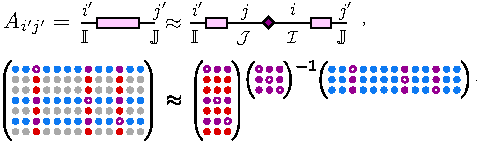
\includegraphics[width=.65\textwidth]{figures/AMCI_IndexSets.pdf}};
		\node[anchor=north east] at (img.north east){\footnotemark};
	\end{tikzpicture}
	\nonumber
\end{gather}

\footnotetext{We introduce here a tensor network diagrammatic representation of the matrix multiplication. The internal connecting solid lines represent summation over the respective matrix indices, according to the \textit{Einstein summation convention}. The external lines represent fixed indices.}

\prettyref{eq:MCI} gives a rank-$\tchi$ approximation of $A$, where $\tchi = \text{dim}\left( \mathcal{I} \right) = \text{dim}\left( \mathcal{J} \right)$. CI is ``only'' a quasioptimal decomposion of $A$ and its accuracy strongly depends on the choice of the pivots; however, contrarily to its optimal counterparts (e.g. SVD), it doesn't require knowing (and saving in memory) the full $M \times N$ matrix to be computed. Let's consider the following example: 
\begin{example}[$5 \times 5$ Correlation matrix]
\label{ex:CIcorrmat}
For classical Harmonic Oscillator 1D chain mode-like vectors: 

\[
\begin{alignedat}{2}      
	\boldsymbol{v} = \frac{\boldsymbol{1}_5}{\sqrt{5}} \qquad \boldsymbol{w} = \frac{(-2,-1,\dots,2)}{2\sqrt{5}}
\end{alignedat}
\]
the corresponding position-position correlation matrix can be ``cross interpolated'' as 

\begin{gather}
	\nonumber \begin{aligned}
		& C  \;=\; \sigma^2 \boldsymbol{v}^T \boldsymbol{v} + \tilde{\sigma}^2 \boldsymbol{w}^T\boldsymbol{w} = \\[.4em]
		& =\frac{1}{115}%
		\begin{tikzpicture}[baseline=-0.5ex,
			every node/.style={inner sep=1pt,font=\small}]
			\matrix (M) [matrix of math nodes,
			nodes={text width=1.8cm, align=center,
			minimum height=1.5em, anchor=center},
			column 1/.style= {nodes={fill=red!30}},
			column 5/.style= {nodes={fill=red!30}},
			row 1/.style= {nodes={fill=yellow!30}},
			row 5/.style= {nodes={fill=yellow!30}},
			row 1 column 1/.style={nodes={fill=orange!30}},
			row 1 column 5/.style={nodes={fill=orange!30}},
			row 5 column 1/.style={nodes={fill=orange!30}},
			row 5 column 5/.style={nodes={fill=orange!30}},
			left delimiter={[},right delimiter={]}, text width=1.8cm,
			ampersand replacement=\&] {
				23\sigma^{2}+72\tilde\sigma^{2} \& 23\sigma^{2}-18\tilde\sigma^{2}
				\& 23\sigma^{2}+12\tilde\sigma^{2}
				\& 23\sigma^{2}-18\tilde\sigma^{2}
				\& 23\sigma^{2}-48\tilde\sigma^{2}\\
				\cdots \& 23\sigma^{2}+{\tfrac92}\tilde\sigma^{2}
				\& 23\sigma^{2}-3\tilde\sigma^{2}
				\& 23\sigma^{2}+{\tfrac92}\tilde\sigma^{2}
				\& 23\sigma^{2}+12\tilde\sigma^{2}\\
				\cdots \& \cdots
				\& 23\sigma^{2}+2\tilde\sigma^{2}
				\& 23\sigma^{2}-3\tilde\sigma^{2}
				\& 23\sigma^{2}-8\tilde\sigma^{2}\\
				\cdots \& \cdots \& \cdots
				\& 23\sigma^{2}+{\tfrac92}\tilde\sigma^{2}
				\& 23\sigma^{2}+12\tilde\sigma^{2}\\
				\cdots \& \cdots \& \cdots \& \cdots
				\& 23\sigma^{2}+32\tilde\sigma^{2}\\
				};
			\draw [decorate, line width=1.5pt,
				decoration = {calligraphic brace,mirror,raise=5pt, amplitude=5pt}] (M.south west) --  (M.south east) node[pos=0.5, below=12pt]{\normalsize $5 \times 5$};
		\end{tikzpicture}
	\end{aligned}
	 \\[1.2em]
	  \approx
	   \underbrace{%
	  C[\mathds{I} , \mathcal{J}]}_{\displaystyle 5 \times 2}
	\,
	\underbrace{%
	  \left[ \begin{array}{>{\columncolor{orange!30}}c>{\columncolor{orange!30}}c}
		\frac{23\sigma^2 + 72\tilde{\sigma}^2}{115} & \frac{23\sigma^2  -48 \tilde{\sigma}^2}{115} \\[0.2em]
		\frac{23\sigma^2 - 48\tilde{\sigma}^2}{115} & \tikzmark{m2}{\frac{23\sigma^2 + 32\tilde{\sigma}^2}{115}}
	  \end{array}\right]^{-1}}_{\displaystyle 2 \times 2}
	  \,
	  \underbrace{%
	  C[\mathcal{I} , \mathds{J}]}_{\displaystyle 5 \times 2}
\end{gather}

with $\sigma$ and $\tilde{\sigma}$ the variances of the two modes and $\mathcal{I} = \{ 1,5\}$ and $\mathcal{J} = \{ 1,5\}$. From the definition of $C$ we can recognize that $\rank{C} = 2$. This property is correctly highlighted by its CI decomposition ($\dim \mathcal{I} = \dim \mathcal{J} = 2$), since, in this particular case, the approximation is exact (cf. \prettyref{prop:CI}-\hyperlink{cond:rankexact}{3.}). The total number of floating point numbers necessary to store the whole matrix in memory is $5 \times 5 = 25$, while for the CI decomposition $5\times 2 \times 2 + 2\times 2 = 24$ are sufficient. It is easy to deduce that the reduction in memory costs becomes less derisory for modes of generic dimension $N$ ($N\times N \gg N \times 2 \times 2 + 2\times 2$ when $N \gg 1$).
\end{example}

From the example above we can evince the computational advantage of CI, however -- in order to make such approximation computationally feasable -- some sort error control is necessary. 
In particular, the error of the CI approximation is related to the \textit{Schur complement} of the matrix to interpolate \cite{Golub96}. 

\begin{definition}[Schur Complement]
	Let us partition a matrix $A\in\mathds{K}^{M\times N}$ ($\mathds{K} = \mathds{R}, \mathds{C}$) in blocks as follows: 

	\begin{equation}
		\begin{bNiceMatrix}[last-row, last-col]
			A_{11} & A_{12} & {\scriptstyle \tchi} \\
			A_{21} & A_{22} & {\scriptstyle M - \tchi} \\
			{\scriptstyle \tchi} & {\scriptstyle N - \tchi}
		\end{bNiceMatrix}.
	\end{equation}
The {\normalfont \textbf{Schur complement}} $[A/A_{11}]$ of $A$ is defined by 
	\begin{equation}
		\label{eq:Schurcomp}
		[A/A_{11}] = A_{22} - A_{21}(A_{11})^{-1}A_{12}.
	\end{equation}
\end{definition}

\begin{proposition}
	\label{prop:CI}
	The following properties hold for a rank-$\tchi$ Cross Interpolation decomposition of a matrix $A$: 

	\begin{enumerate}
		\item the error of CI is given by the Schur complement to the pivot matrix;
		\item the approximation is exact for any $i \in \mathcal{I}$ or $j \in \mathcal{J}$; 
		\item \hypertarget{cond:rankexact} the approximation is exact if $A$ has rank $\tchi$.
	\end{enumerate}
	 
\end{proposition}\vspace{-10pt}
\begin{proof}
	\textit{1.-2.} - The Schur complement is invariant under rows and/or column permutations, therefore let us rearrange $A = A[\mathds{I}, \mathds{J}]$ such that
	\begin{equation*}
		A = \begin{bmatrix}
			A[\mathcal{I}, \mathcal{J}] & A[\mathcal{I}, \mathds{J} / \mathcal{J}] \\
			A[\mathds{I} / \mathcal{I}, \mathcal{J}]  & A[\mathds{I} / \mathcal{I}, \mathds{J} / \mathcal{J}]  
		\end{bmatrix}.
	\end{equation*}
Then, \prettyref{eq:MCI} can be rewritten as 
	\begin{equation*}
		\tilde{A} = \begin{bmatrix}
			A[\mathcal{I}, \mathcal{J}] & A[\mathcal{I}, \mathds{J} / \mathcal{J}] \\
			A[\mathds{I} / \mathcal{I}, \mathcal{J}]  &   A[\mathds{I} / \mathcal{I}, \mathcal{J}] \left(A[\mathcal{I}, \mathcal{J}] \right)^{-1} A[\mathcal{I}, \mathds{J} / \mathcal{J}]
		\end{bmatrix}
	\end{equation*}
	which gives (cf. Ref. \cite{Fernandez2024})
	\begin{equation}
		A - \tilde{A} = \begin{bmatrix}
			0 & 0 \\
			0 & [A/A[\mathcal{I}, \mathcal{J}]]
		\end{bmatrix}
	\end{equation}
\textit{3.} - If $\rank{A} = \tchi$ and $P = A[\mathcal{I},\mathcal{J}]$ is non-singular, then 

\begin{equation}
	\begin{bmatrix}
		A[\mathcal{I}, \mathcal{J}] & A[\mathcal{I},j] \\
		A[i, \mathcal{J}] & A[i,j]
	\end{bmatrix}\qquad \forall\; (i,j) \in \mathds{I} / \mathcal{I} \times \mathds{J} / \mathcal{J}
\end{equation}
is singular, which gives $ A[i,j] = A[i, \mathcal{J}] \left( A[\mathcal{I}, \mathcal{J}] \right)^{-1} A[\mathcal{I},j]$ (cf. App A-B in Ref. \cite{Fernandez2022}). 
\end{proof}

\prettyref{prop:CI} underlines the importance of the choice of the pivots and of the pivot matrix, specifically with the purpose of minimizing the Schur complement $[A/A[\mathcal{I}, \mathcal{J}]]$. Such procedure is equivalent to maximising $\det{A[\mathcal{I}, \mathcal{J}]}$ and is known as the \textit{maximum volume principle} \cite{Goreinov1997}. Moreover, from this analysis, we can also get an intuition about why the CI approximation error is at most $O(\tchi^2)$ times the optimal one (e.g. $\tchi$-truncated SVD error) \cite{Schneider2010}, while requiring only subparts of the original matrix to be known. 

\subsubsection{Partial rank-revealing LU decomposition (prrLU)}
Matrix Cross Interpolation presents itself as a very useful tool when it comes to numerical compression of matrices. Generalization of CI to continuous domains \cite{Schneider2010, Fernandez2022} even allows for reduction of numerical complexity of integration and derivation. Nonetheless, for practical, very complex, calculations, CI starts to fail. Numerical instability issues like rounding errors, ill-conditioning or overflowing \cite{Golub96} easily emerge when CI requires large values of $\tchi$ to be accurate, therefore making the pivot matrix \textit{almost singular}. 

Partial rank-revealing LU (prrLU) \cite{Golub96, Pan2000} matrix decomposition proposes itself as a possible solution for the numerical fragilities of CI. The prrLU provides a more stable, but equivalent approximation of our matrix to decompose. While avoiding any inversion of the pivot matrix $A[\mathcal{I}, \mathcal{J}]$, similarly to CI, prrLU only requires a small subset of matrix's elements to be known. 

We may summarize the main features of prrLU as follows:

\begin{itemize}
	\item prrLU is \textit{rank revealing}, i.e. it allows for the determination of the rank of the decomposed matrix;
	\item prrLU is \textit{partial} (and therefore \textit{controllable}), i.e. the decomposition is stopped after constructing the first $\tchi$ rows of $L$ and columns of $U$, for a fixed $\tchi$;
	\item prrLU is \textit{updatable}, i.e. given pivot lists $\mathcal{I}, \mathcal{J}$ yielding an approximation $\tilde{A}$ of $A$, new rows and columns can easily be added to $\mathcal{I}, \mathcal{J}$ for an improved approximation. 
\end{itemize}

The prrLU implementation relies on the following LU decomposition (easily inferred from \prettyref{eq:Schurcomp}):

\begin{gather}
	\label{eq:SchurLU}
	\begin{bmatrix}
	A_{11} & A_{12} \\
	A_{21} & A_{22}
	\end{bmatrix}
	%\nonumber \\
	=
	\begin{bmatrix}
	L_{11} & 0 \\
	L_{21} & \identity_{22}
	\end{bmatrix}
	\begin{bmatrix}
	A_{11} & 0 \\
	0 & [A / A_{11}]
	\end{bmatrix}
	\begin{bmatrix}
	U_{11} & U_{12} \\
	0 & \identity_{22}
	\end{bmatrix}\\[6pt]
	\nonumber L_{11} = U_{11} = \identity_{11}, \qquad L_{21} = A_{21}A^{-1}_{11}, \qquad U_{12} = A^{-1}_{11}A_{12}
\end{gather} 
From \prettyref{eq:SchurLU} we can already understand where the improved stability of prrLU comes from: no matrix inversion is computed directly! The general prrLU routine proceeds as outlined below:  

\begin{algorithm}[H]
	\caption{Partial rank revealing LU}
	\label{alg:prrLU}
    \SetKwFunction{findBestPivot}{findBestPivot}
	\SetKwFunction{strictlyLowerTriangular}{strictlyLowerTriangular}
	\SetKwFunction{strictlyUpperTriangular}{strictlyUpperTriangular}
    \SetKwInOut{KwIn}{Input}
    \SetKwInOut{KwOut}{Output}

    \KwIn{$A\in\mathds{K}^{M\times N}$ matrix, max rank $\tchi$ and tolerance $\varepsilon$. }
    \KwOut{Rows permutation $\Pi_r$, columns permutation $\Pi_c$, $L$, $U$, $N_{pivots}$}

    $\Pi_r\leftarrow(1,\dots,M)$,\quad $\Pi_c\leftarrow(1,\dots,N)$,\quad 
	$n\leftarrow0$,\quad $\varepsilon_{LU} \leftarrow \varepsilon$\;

	\While{$n<\min(\tchi,\,M,\,N)$}{
		$n\leftarrow n+1$\;
		$(r^\star,c^\star)\leftarrow 
		\findBestPivot\!\bigl(A[n\!:\!N, n\!:\!M]\bigr)$\tcp*[f]{current positions}\;
		swap rows $n\leftrightarrow r^\star$ in $A$ and $\Pi_r$\;
		swap cols $n\leftrightarrow c^\star$ in $A$ and $\Pi_c$\;
		$\varepsilon_{LU} \leftarrow |A_{n,n}|$\;
		\If(\tcp*[f]{error test}){$n>0$ \KwSty{and} $\varepsilon_{LU} <\varepsilon$}{
			\textbf{break}\;
		}	
	}
	
	$L\leftarrow\strictlyLowerTriangular\bigl(A[:,\,1\!:\!n]\bigr)$\;
	$U\leftarrow\strictlyUpperTriangular\bigl(A[1\!:\!n,\,:]\bigr)$\;
	\Return{$(\Pi_r,\,\Pi_c,\,L,\,U,\,n)$}\;
\end{algorithm}

By iteratively applying \prettyref{eq:SchurLU} on the lower-right block of the internal matrix, while limiting $A_{11}$ to a $1\times 1$ submatrix, \prettyref{alg:prrLU} allows us to obtain an approximation of the form 

\begin{equation}
	A = LDU + \begin{bmatrix}
		0 & 0\\
		0 & [A/A[\mathcal{I}, \mathcal{J}]]
	\end{bmatrix} = \tilde{A} + \textrm{err.},
\end{equation}

perfectly equivalent to \prettyref{eq:MCI} (cf. Ref. \cite{Fernandez2024}), where $D$ is a diagonal matrix containing -- after iterative permutations -- the first $\tchi$ optimal pivots of $A$.
Some remarks about \prettyref{alg:prrLU} are in order: 
\begin{itemize}
	\item the implementation of prrLU is based upon the search of a good \textit{pivot} (\texttt{findBestPivot}). Through the \textit{maxvol principle}, a good pivot is defined as one that maximises the volume of the submatrix $A[\mathcal{I}, \mathcal{J}]$ ($\equiv A_{11}$ after permutation). The iterative application of \prettyref{eq:SchurLU} reduces the optimization pivot to the largest element of the submatrix $A[n\!:\!N, n\!:\!M]$ at iteration $n$;
	\item different strategies can be implemented for pivot searching; a naive approach consists in a \textit{full search} scheme scanning the entire submatrix. $O(MN)$ poor scaling of the naive implementation renders prrLU computationally inefficient. \textit{Rook search} \cite{Poole2000} and \textit{block rook search} \cite{Fernandez2024} are cleverer and cheaper approaches, with comparable robutstness and convergence, but reduced computational cost $O(\max\left(M,N\right))$;  
	\item the matrix elements explored during \textit{rook search} are sufficient to perform prrLU of $A$. Therefore, prrLU yields compressibility features similar to those of CI (see Example \ref{ex:CIcorrmat}). For this reason, prrLU can also be applied to 2-dimensional functions discretized on a grid, whose full structure is uknown a priori; 	
	\item the absolute error of the prrLU approximation is reduced to the modulus of the last inserted pivot, as one can understand from \prettyref{alg:prrLU}. The reason behind this is that we intend to minimize $\parallel\! A - \tilde{A}\!\parallel_{\textrm{max}} = \parallel\![A/A[\mathcal{I}, \mathcal{J}]] \!\parallel_{\textrm{max}}$ which is bounded by $\parallel\! A[n_{\textrm{end}}\!:\!N, n_{\textrm{end}}\!:\!M]\!\parallel_{\textrm{max}}$ of the last iteration.  
\end{itemize}


\subsection{Tensor Cross Interpolation}

The number of function calls necessary to construct $\widetilde{\mathcal{T}}$ from $\mathcal{T}$ is $O(\mathcal{L}d\chi^2) \ll d^\mathcal{L}$, fully specifying only $O(\mathcal{L}\chi^2)$ number of \textit{pivots}.

The TCI algorithm computational time scales as $O(\mathcal{L}d\chi^2)$. 

\begin{definition}
	A function $f$ is {\normalfont \textbf{almost separable}} if its tensor approximation $F$ is \underline{low-rank}.
	\label{def:separfunc}
\end{definition}


\note{Tensor Cross Interpolation}{Main paper: \cite{Fernandez2024}, Main TCI ref: \cite{Oseledets2010}, polynomial dimension scaling, matrix cross interpolation \cite{Goreinov1997}, function learning, N-dimensional integrals, \textit{$\epsilon$-factorizability} of continuous functions $\to$ reduction from N to one-dimensional integrals independent of function sign ($\int \text{d}\mathbf{x} f(x_1, ... , x_N) \approx \prod\limits_{\alpha = 1 }^N\int \text{d}x_1 T_\alpha(x_\alpha)P_\alpha^{-1}$) and $|| f - f_\text{TCI} || < \epsilon $, N-dimensional integral $O(\mathcal{L}d\chi^2)$ (not $d^\mathcal{L}$) , tensor representation $O(\mathcal{L}\chi^2)$ (??), \textit{active machine learning} \cite{Settles2012}: find the region with the largest approximation error, main challenge: bookkeeping and notation, \textit{maxvol} principle \cite{Dolgov2020}, exact if $\rank{TT} = \chi$ like MCI (see Naive Approach \cite{Fernandez2022}), \textit{multi-indices} and \texttt{Vector}\{\textit{multi-indices}\}, $\bigoplus$= concatenation of multi-indices, \textit{nesting condition} \cite{Oseledets2011,Dolgov2020}$\to$ $\mathcal{I}_\alpha \subset \mathcal{I}_{\alpha -1 } \bigoplus \mathds{K}_\alpha$ and $\mathcal{J}_\alpha \subset \mathds{K}_\alpha \bigoplus \mathcal{J}_{\alpha +1 }$(this guarantees exact interpolation for $f$(pivots)), function calls: $O(\mathcal{L}d\chi^2) \ll d^\mathcal{L}$, $\Pi_\alpha$ and the \textit{error function} $\epsilon_\Pi = |f - f_\text{TCI}|(i, x_\alpha, x_{\alpha +1}, j)$ $\to$ find the maximum of $\epsilon_\Pi$ before adding new pivots (add the pivots that yields the largest improvement of the local accuracy), pivot search: \textit{full}, \textit{rook}, \textit{block-rook}, \textit{alternate}(alternate:single pivot $O(d\chi)$, total search $O(d\chi^2)$ \cite{Fernandez2022}), \textit{environment-aware} $\epsilon_\Pi$ $\to$ error function related to the error of the integral that takes in consideration the volume contribution to the integral, \textit{environment} vectors $L_i$ and $R_j$, \textit{rank-revealing} (only slow convergence for high rank), \textit{polynomial costs}, integration scales $1/N_{eval}$ compared to $1/\sqrt{N_{eval}}$ Monte Carlo (cf. Ref. \cite{Fernandez2024} Fig. 2); separation of pivot exploration and tensor update could be beneficial (see Monte Carlo \textit{space configuration enlargment})}\\


\note{Applications}{Feynmann diagramm expansion \cite{Fernandez2022}: high-order real-time nonequilibrium Schwinger-Keldysh perturbation expansions (integral convergence $1/N^2$, $N$ function evaluations), multi-dimensional function minimization and quantized reinforcement learning \cite{Sozykin2022} (outperfoming standardized gradient-free methods in number of function evaluations and execution time), computation of Brilloin zone integrals to calculate topological invariants \cite{Ritter2024}, compact tensorization of atomic orbitals bases with high accuracy \cite{Jolly2024} (error on energy of \ce{H2} improved by 85\% w.r.t. double zeta calculation), speed-up of multi-assets Fourier transform-based option pricing \cite{Sakurai2025}}\\

\noindent\note{Nice sentences}{The approximation is systematically controlled by $\chi$. TCI is a generalization of the matrix cross interpolation to $N$-dimensional tensors and functions. Summation is implicit over the indices connecting two  tensors. TCI representation is defined by the selected $\mathcal{I}$ and $\mathcal{J}$, so an accurate interpolation amounts to optimizing this selection. TCI approximation of $f$ is built from one-dimensional slices  of $f$. Tensor network methods offer a new appraoch to high-dimensional integration. It significantly outperform Monte-Carlo and quasi-Monte-Carlo methods in differente applications. The limiting factor of TCI (rank of the $\epsilon$-factorization) is entirely orthogonal to that of sampling methods. The tensor cross interpolation (TCI) algorithm is a rank-revealing algorithm for decom-
posing low-rank, high-dimensional tensors into tensor trains/matrix product states (MPS).}\\

\noindent\note{General references}{\cite{Oseledets2010, Oseledets2011, Savostyanov2014, Savostyanov2011, Dolgov2020}}\\
\note{Open questions}{Generality of $\epsilon$-factorizability property}

\subsection{The Quantics Representation: QTCI}



\note{QTCI}{Discards weak entanglement between different scales; works well for scale-separated, non-irregular functions; $O(\mathcal{L} \log N )$ ($N \stackrel{?}{=} 2^R $) quantics approximation scaling 4 $\to$ logarithmic scaling in the number of grid points \cite{Khoromskij2011}; exponentially high resolution; low-rank scale separated structure revealed through TCI + quantics }\\

\noindent \note{Nice Sentences}{Numerical computations with multivariate functions typically involve a compromise between two contrary desiderata: accurate resolution of the functional dependence, versus parsimonious memory usage.}\\

\noindent \note{General references}{\cite{Oseledets2009} (quantics and interleaved representation) }\\

\noindent \note{Applications}{Approximation and manipulation of correlation functions for quantum many body systems \cite{Hiroshi2023}; compression of imaginary-time propagators in the Frobenious norm \cite{Takahashi2025}; diagrammatic non-equilibrium many-body Green’s function-based calculations \cite{Murray2024} $\to$ better scaling of resourses for higher precisions $R$ or longer times }\\

\noindent \note{Open questions 
}{When does a multivariate function admit low-rank representation? }





\section{Computational Fallbacks: Localised Functions}

\begin{figure}[ht!]
	\caption{2D: Heatmap + error Heatmap of TCI approximation of a very localised function with different zoomings  }
\end{figure}

\subsection{Localised Function and Memory Consumption}

\begin{figure}[ht!]
	\caption{1D: plot of different patch subdivision and relative bond dimension per patch for each division (like patching paper)  }
\end{figure}

\begin{figure}[ht!]
	\caption{2D: Bond dimension vs bond for each of the zoomings and for one of the more trivial parts of the function. }
\end{figure}

